\documentclass[]{article}
\usepackage{lmodern}
\usepackage{amssymb,amsmath}
\usepackage{ifxetex,ifluatex}
\usepackage{fixltx2e} % provides \textsubscript
\ifnum 0\ifxetex 1\fi\ifluatex 1\fi=0 % if pdftex
  \usepackage[T1]{fontenc}
  \usepackage[utf8]{inputenc}
\else % if luatex or xelatex
  \ifxetex
    \usepackage{mathspec}
  \else
    \usepackage{fontspec}
  \fi
  \defaultfontfeatures{Ligatures=TeX,Scale=MatchLowercase}
\fi
% use upquote if available, for straight quotes in verbatim environments
\IfFileExists{upquote.sty}{\usepackage{upquote}}{}
% use microtype if available
\IfFileExists{microtype.sty}{%
\usepackage{microtype}
\UseMicrotypeSet[protrusion]{basicmath} % disable protrusion for tt fonts
}{}
\usepackage[margin=1in]{geometry}
\usepackage{hyperref}
\hypersetup{unicode=true,
            pdftitle={Course 7 - Regression Models Project},
            pdfauthor={Grejell Segura},
            pdfborder={0 0 0},
            breaklinks=true}
\urlstyle{same}  % don't use monospace font for urls
\usepackage{color}
\usepackage{fancyvrb}
\newcommand{\VerbBar}{|}
\newcommand{\VERB}{\Verb[commandchars=\\\{\}]}
\DefineVerbatimEnvironment{Highlighting}{Verbatim}{commandchars=\\\{\}}
% Add ',fontsize=\small' for more characters per line
\usepackage{framed}
\definecolor{shadecolor}{RGB}{248,248,248}
\newenvironment{Shaded}{\begin{snugshade}}{\end{snugshade}}
\newcommand{\KeywordTok}[1]{\textcolor[rgb]{0.13,0.29,0.53}{\textbf{#1}}}
\newcommand{\DataTypeTok}[1]{\textcolor[rgb]{0.13,0.29,0.53}{#1}}
\newcommand{\DecValTok}[1]{\textcolor[rgb]{0.00,0.00,0.81}{#1}}
\newcommand{\BaseNTok}[1]{\textcolor[rgb]{0.00,0.00,0.81}{#1}}
\newcommand{\FloatTok}[1]{\textcolor[rgb]{0.00,0.00,0.81}{#1}}
\newcommand{\ConstantTok}[1]{\textcolor[rgb]{0.00,0.00,0.00}{#1}}
\newcommand{\CharTok}[1]{\textcolor[rgb]{0.31,0.60,0.02}{#1}}
\newcommand{\SpecialCharTok}[1]{\textcolor[rgb]{0.00,0.00,0.00}{#1}}
\newcommand{\StringTok}[1]{\textcolor[rgb]{0.31,0.60,0.02}{#1}}
\newcommand{\VerbatimStringTok}[1]{\textcolor[rgb]{0.31,0.60,0.02}{#1}}
\newcommand{\SpecialStringTok}[1]{\textcolor[rgb]{0.31,0.60,0.02}{#1}}
\newcommand{\ImportTok}[1]{#1}
\newcommand{\CommentTok}[1]{\textcolor[rgb]{0.56,0.35,0.01}{\textit{#1}}}
\newcommand{\DocumentationTok}[1]{\textcolor[rgb]{0.56,0.35,0.01}{\textbf{\textit{#1}}}}
\newcommand{\AnnotationTok}[1]{\textcolor[rgb]{0.56,0.35,0.01}{\textbf{\textit{#1}}}}
\newcommand{\CommentVarTok}[1]{\textcolor[rgb]{0.56,0.35,0.01}{\textbf{\textit{#1}}}}
\newcommand{\OtherTok}[1]{\textcolor[rgb]{0.56,0.35,0.01}{#1}}
\newcommand{\FunctionTok}[1]{\textcolor[rgb]{0.00,0.00,0.00}{#1}}
\newcommand{\VariableTok}[1]{\textcolor[rgb]{0.00,0.00,0.00}{#1}}
\newcommand{\ControlFlowTok}[1]{\textcolor[rgb]{0.13,0.29,0.53}{\textbf{#1}}}
\newcommand{\OperatorTok}[1]{\textcolor[rgb]{0.81,0.36,0.00}{\textbf{#1}}}
\newcommand{\BuiltInTok}[1]{#1}
\newcommand{\ExtensionTok}[1]{#1}
\newcommand{\PreprocessorTok}[1]{\textcolor[rgb]{0.56,0.35,0.01}{\textit{#1}}}
\newcommand{\AttributeTok}[1]{\textcolor[rgb]{0.77,0.63,0.00}{#1}}
\newcommand{\RegionMarkerTok}[1]{#1}
\newcommand{\InformationTok}[1]{\textcolor[rgb]{0.56,0.35,0.01}{\textbf{\textit{#1}}}}
\newcommand{\WarningTok}[1]{\textcolor[rgb]{0.56,0.35,0.01}{\textbf{\textit{#1}}}}
\newcommand{\AlertTok}[1]{\textcolor[rgb]{0.94,0.16,0.16}{#1}}
\newcommand{\ErrorTok}[1]{\textcolor[rgb]{0.64,0.00,0.00}{\textbf{#1}}}
\newcommand{\NormalTok}[1]{#1}
\usepackage{graphicx,grffile}
\makeatletter
\def\maxwidth{\ifdim\Gin@nat@width>\linewidth\linewidth\else\Gin@nat@width\fi}
\def\maxheight{\ifdim\Gin@nat@height>\textheight\textheight\else\Gin@nat@height\fi}
\makeatother
% Scale images if necessary, so that they will not overflow the page
% margins by default, and it is still possible to overwrite the defaults
% using explicit options in \includegraphics[width, height, ...]{}
\setkeys{Gin}{width=\maxwidth,height=\maxheight,keepaspectratio}
\IfFileExists{parskip.sty}{%
\usepackage{parskip}
}{% else
\setlength{\parindent}{0pt}
\setlength{\parskip}{6pt plus 2pt minus 1pt}
}
\setlength{\emergencystretch}{3em}  % prevent overfull lines
\providecommand{\tightlist}{%
  \setlength{\itemsep}{0pt}\setlength{\parskip}{0pt}}
\setcounter{secnumdepth}{0}
% Redefines (sub)paragraphs to behave more like sections
\ifx\paragraph\undefined\else
\let\oldparagraph\paragraph
\renewcommand{\paragraph}[1]{\oldparagraph{#1}\mbox{}}
\fi
\ifx\subparagraph\undefined\else
\let\oldsubparagraph\subparagraph
\renewcommand{\subparagraph}[1]{\oldsubparagraph{#1}\mbox{}}
\fi

%%% Use protect on footnotes to avoid problems with footnotes in titles
\let\rmarkdownfootnote\footnote%
\def\footnote{\protect\rmarkdownfootnote}

%%% Change title format to be more compact
\usepackage{titling}

% Create subtitle command for use in maketitle
\newcommand{\subtitle}[1]{
  \posttitle{
    \begin{center}\large#1\end{center}
    }
}

\setlength{\droptitle}{-2em}
  \title{Course 7 - Regression Models Project}
  \pretitle{\vspace{\droptitle}\centering\huge}
  \posttitle{\par}
  \author{Grejell Segura}
  \preauthor{\centering\large\emph}
  \postauthor{\par}
  \predate{\centering\large\emph}
  \postdate{\par}
  \date{8/21/2017}


\begin{document}
\maketitle

\subsection{Excutive Summary}\label{excutive-summary}

This report investigated the difference of manual and automatic
transmission cars by looking at their miles/galloon measures. Other
variables are also investigated to find possible interactions and
confounding effects. The data used is the mtcars taken from the package
``datasets''.

\paragraph{Load Libraries}\label{load-libraries}

I used a number of libraries to help me with the visualizations and
testing.

\begin{Shaded}
\begin{Highlighting}[]
\KeywordTok{library}\NormalTok{(ggplot2)}
\KeywordTok{library}\NormalTok{(datasets)}
\KeywordTok{library}\NormalTok{(gridExtra)}
\KeywordTok{library}\NormalTok{(corrplot)}
\KeywordTok{library}\NormalTok{(car)}
\KeywordTok{library}\NormalTok{(lmtest)}
\KeywordTok{library}\NormalTok{(caret)}
\end{Highlighting}
\end{Shaded}

\subsubsection{Exploratory Data
Analysis}\label{exploratory-data-analysis}

First, let us check the data structure.

\begin{Shaded}
\begin{Highlighting}[]
\KeywordTok{dim}\NormalTok{(mtcars)}
\end{Highlighting}
\end{Shaded}

\begin{verbatim}
## [1] 32 11
\end{verbatim}

The data has 32 observations with 11 variables.

Now let us convert some of the variables to factors.

\begin{Shaded}
\begin{Highlighting}[]
\NormalTok{mtcars[, }\KeywordTok{c}\NormalTok{(}\StringTok{"cyl"}\NormalTok{, }\StringTok{"vs"}\NormalTok{, }\StringTok{"am"}\NormalTok{, }\StringTok{"gear"}\NormalTok{, }\StringTok{"carb"}\NormalTok{)] <-}\StringTok{ }\KeywordTok{lapply}\NormalTok{(mtcars[, }\KeywordTok{c}\NormalTok{(}\StringTok{"cyl"}\NormalTok{, }\StringTok{"vs"}\NormalTok{, }\StringTok{"am"}\NormalTok{, }\StringTok{"gear"}\NormalTok{, }\StringTok{"carb"}\NormalTok{)], as.factor)}
\end{Highlighting}
\end{Shaded}

Then let us examine the data by looking at the summary of am and mpg.

\begin{Shaded}
\begin{Highlighting}[]
\KeywordTok{summary}\NormalTok{(mtcars}\OperatorTok{$}\NormalTok{mpg)}
\end{Highlighting}
\end{Shaded}

\begin{verbatim}
##    Min. 1st Qu.  Median    Mean 3rd Qu.    Max. 
##   10.40   15.42   19.20   20.09   22.80   33.90
\end{verbatim}

\begin{Shaded}
\begin{Highlighting}[]
\KeywordTok{var}\NormalTok{(mtcars}\OperatorTok{$}\NormalTok{mpg)}
\end{Highlighting}
\end{Shaded}

\begin{verbatim}
## [1] 36.3241
\end{verbatim}

\begin{Shaded}
\begin{Highlighting}[]
\KeywordTok{summary}\NormalTok{(mtcars}\OperatorTok{$}\NormalTok{am)}
\end{Highlighting}
\end{Shaded}

\begin{verbatim}
##  0  1 
## 19 13
\end{verbatim}

Looking at the mpg summary, the mean is 20.09 with variance of 36.3241.
As for the variable am, there are 19 cars classified as automatic while
13 are manual.

To have an initial insight, it is best to visualize the data. We will
focus first on mgp and am variables as this is our main concern on this
problem. The result can be in Figure 1 below.

\begin{center}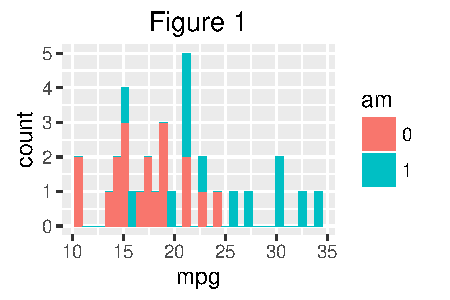
\includegraphics{Course_7_Week_4_Regression_Models_files/figure-latex/unnamed-chunk-5-1} \end{center}

Figure 1 shows the distribution of mpg broken down per transmission
type. We can see that there is some sort of separation between 2
transmission types where automatic transmission has higher median.

Another chart was created to examine the relationship of mpg to other
categorical variables. The result is showed in the Appendix section as
Figure 2. Looking at the figure, we can see that there is also some sort
of separation between mpg vs.~cyl, mpg vs.~vs, and mpg vs.~gear. As for
mpg vs.~carb, there is no clear separation to it.

We are done visualizing and examining mpg against the categorical
variables. Next is we try to see if it also has some sort of relation
with respect to the numerical variables. Let us see by looking at the
correlation graph below.

\begin{Shaded}
\begin{Highlighting}[]
\NormalTok{cor <-}\StringTok{ }\KeywordTok{cor}\NormalTok{(mtcars[, }\KeywordTok{c}\NormalTok{(}\StringTok{"mpg"}\NormalTok{, }\StringTok{"disp"}\NormalTok{, }\StringTok{"hp"}\NormalTok{, }\StringTok{"drat"}\NormalTok{, }\StringTok{"wt"}\NormalTok{, }\StringTok{"qsec"}\NormalTok{)])}
\NormalTok{cor}
\end{Highlighting}
\end{Shaded}

\begin{verbatim}
##             mpg       disp         hp        drat         wt        qsec
## mpg   1.0000000 -0.8475514 -0.7761684  0.68117191 -0.8676594  0.41868403
## disp -0.8475514  1.0000000  0.7909486 -0.71021393  0.8879799 -0.43369788
## hp   -0.7761684  0.7909486  1.0000000 -0.44875912  0.6587479 -0.70822339
## drat  0.6811719 -0.7102139 -0.4487591  1.00000000 -0.7124406  0.09120476
## wt   -0.8676594  0.8879799  0.6587479 -0.71244065  1.0000000 -0.17471588
## qsec  0.4186840 -0.4336979 -0.7082234  0.09120476 -0.1747159  1.00000000
\end{verbatim}

Looking at the correlation table, mpg has high negative correlation with
disp, hp, and wt. On the other hand, drat has relatively high positive
correlation with mpg, qsec meanwhile has the lowest correlation with
mpg.

\subsection{Inferential Analysis}\label{inferential-analysis}

Let us now examine the relationships by having an inferential analysis.
The main objective is to see if there is an evidence of the difference
of 2 types of transmission. We also want to quantify this effect by
fitting a model.

We will use a t-test to determine if there is an evidence of difference
in the mpg means for the 2 different types. Looking back at the graph,
we have an assumption that automatic transmission has more mpg mean so
we will have the hypothesis testing in this manner.\\
Ho : there is no difference of mpg means between 2 types of
transmissions Ha : automatic transmission has greater mean than manual
transmission

\begin{Shaded}
\begin{Highlighting}[]
\NormalTok{model.}\DecValTok{1}\NormalTok{ <-}\StringTok{ }\KeywordTok{t.test}\NormalTok{(mpg }\OperatorTok{~}\StringTok{ }\NormalTok{am, mtcars, }\DataTypeTok{alternative =} \StringTok{"greater"}\NormalTok{)}
\NormalTok{model.}\DecValTok{1}
\end{Highlighting}
\end{Shaded}

\begin{verbatim}
## 
##  Welch Two Sample t-test
## 
## data:  mpg by am
## t = -3.7671, df = 18.332, p-value = 0.9993
## alternative hypothesis: true difference in means is greater than 0
## 95 percent confidence interval:
##  -10.57662       Inf
## sample estimates:
## mean in group 0 mean in group 1 
##        17.14737        24.39231
\end{verbatim}

The t-test result shows p-value = 0.00069 which very small. Hence we
reject the null hypothesis and declare that there is a statistical
difference between the 2 transmissions and that automatic transmission
has greater mpg mean than its manual counterpart. Ofcourse we dont want
to stop the investigation at this point as we also wish to quantify the
proven difference. We proceed by linear modelling.

\begin{Shaded}
\begin{Highlighting}[]
\NormalTok{model.}\DecValTok{1}\NormalTok{ <-}\StringTok{ }\KeywordTok{lm}\NormalTok{(mpg }\OperatorTok{~}\StringTok{ }\NormalTok{am, mtcars)}
\NormalTok{model.}\DecValTok{1}\OperatorTok{$}\NormalTok{coefficients}
\end{Highlighting}
\end{Shaded}

\begin{verbatim}
## (Intercept)         am1 
##   17.147368    7.244939
\end{verbatim}

The model shows the significance of the coefficient in am1. This means
there is a 7.245 mpg difference between automatic transmission and
manual transmission. However, we should also consider that there are
other confounding variables that may also affect the this effect.
Therefore, we will proceed on creating a model consisting of some of the
variables that may also affect mpg.\\
We wish to build the best model by starting with our model.1 and nesting
it by adding 1 variable at a time. The result is shown in the table
below.

\begin{verbatim}
## Analysis of Variance Table
## 
## Model 1: mpg ~ am
## Model 2: mpg ~ am + cyl
## Model 3: mpg ~ am + cyl + hp
## Model 4: mpg ~ am + cyl + hp + wt
##   Res.Df    RSS Df Sum of Sq      F    Pr(>F)    
## 1     30 720.90                                  
## 2     28 264.50  2    456.40 39.286 1.388e-08 ***
## 3     27 197.20  1     67.30 11.585  0.002164 ** 
## 4     26 151.03  1     46.17  7.949  0.009081 ** 
## ---
## Signif. codes:  0 '***' 0.001 '**' 0.01 '*' 0.05 '.' 0.1 ' ' 1
\end{verbatim}

I stopped adding variables at model.4 as we don't find any significant
difference by adding the remaining variables. Let us examine model.4
then.

\begin{Shaded}
\begin{Highlighting}[]
\KeywordTok{summary}\NormalTok{(model.}\DecValTok{4}\NormalTok{)}
\end{Highlighting}
\end{Shaded}

\begin{verbatim}
## 
## Call:
## lm(formula = mpg ~ am + cyl + hp + wt, data = mtcars)
## 
## Residuals:
##     Min      1Q  Median      3Q     Max 
## -3.9387 -1.2560 -0.4013  1.1253  5.0513 
## 
## Coefficients:
##             Estimate Std. Error t value Pr(>|t|)    
## (Intercept) 33.70832    2.60489  12.940 7.73e-13 ***
## am1          1.80921    1.39630   1.296  0.20646    
## cyl6        -3.03134    1.40728  -2.154  0.04068 *  
## cyl8        -2.16368    2.28425  -0.947  0.35225    
## hp          -0.03211    0.01369  -2.345  0.02693 *  
## wt          -2.49683    0.88559  -2.819  0.00908 ** 
## ---
## Signif. codes:  0 '***' 0.001 '**' 0.01 '*' 0.05 '.' 0.1 ' ' 1
## 
## Residual standard error: 2.41 on 26 degrees of freedom
## Multiple R-squared:  0.8659, Adjusted R-squared:  0.8401 
## F-statistic: 33.57 on 5 and 26 DF,  p-value: 1.506e-10
\end{verbatim}

\begin{Shaded}
\begin{Highlighting}[]
\KeywordTok{AIC}\NormalTok{(model.}\DecValTok{1}\NormalTok{, model.}\DecValTok{2}\NormalTok{, model.}\DecValTok{3}\NormalTok{, model.}\DecValTok{4}\NormalTok{)}
\end{Highlighting}
\end{Shaded}

\begin{verbatim}
##         df      AIC
## model.1  3 196.4844
## model.2  5 168.3989
## model.3  6 161.0033
## model.4  7 154.4669
\end{verbatim}

The summary shows that the model explains 84.01\% of the variance of
mpg. The model also has the lowest Akaike Information Criterion (AIC)
which means it is the best prediction model among the 4 considered.

The following is the residual plots to investigate the goodness of fit
of model.4.

The plots shows that the residuals are randomly scattered and
distributed. This is a good indication.

To make sure, the following diagnostic tests are also considered to see
if the model is good enough.

\begin{Shaded}
\begin{Highlighting}[]
\KeywordTok{dwtest}\NormalTok{(model.}\DecValTok{4}\NormalTok{)}
\end{Highlighting}
\end{Shaded}

\begin{verbatim}
## 
##  Durbin-Watson test
## 
## data:  model.4
## DW = 1.8088, p-value = 0.1567
## alternative hypothesis: true autocorrelation is greater than 0
\end{verbatim}

The dwtest is the Durbin-Watson test which tests the existence of
autocorrelation in the residuals. As observed, the p-value is greater
than 0.5 which means there is no evidence that an autocorrelation exist.

\subsection{Appendix}\label{appendix}

\begin{center}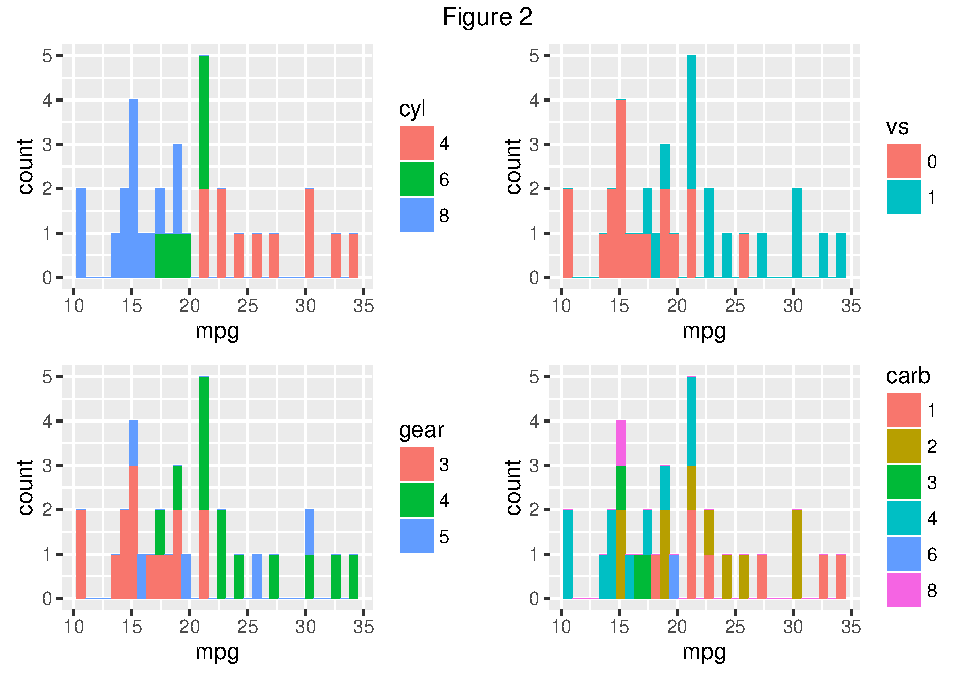
\includegraphics{Course_7_Week_4_Regression_Models_files/figure-latex/unnamed-chunk-13-1} \end{center}


\end{document}
